\section{Mon, Mar 5th}
\subsection{Toy example}
Consider the following economy, 
\[N=\{0,1,2\},\quad E=\{(0,1),(1,2)\},\quad \lambda=5\%,\quad UB=\frac{1}{4},\quad p=\frac{1}{2},\quad a_0=a_1=1,\quad q_0=q_1=q_2=\frac{1}{3},\]
this easy example is depicted in Figure~(\ref{figToyNtw})
\begin{figure}[htbp]
   \centering
   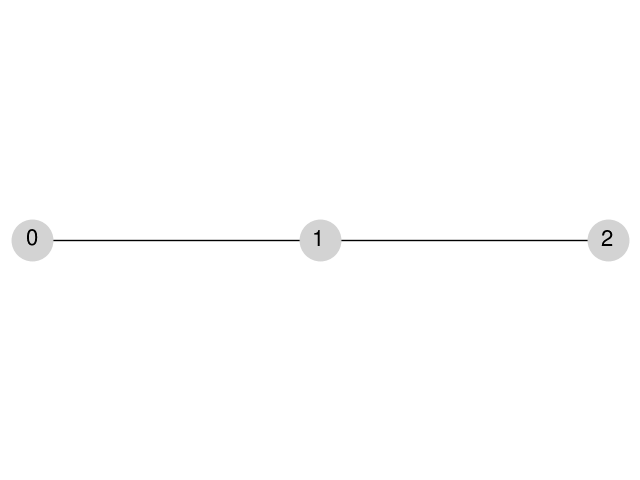
\includegraphics[width=0.9\textwidth]{ToyNtw} % requires the graphicx package
   \caption{Toy example}
   \label{figToyNtw}
\end{figure}
For this economy, we we first compute
\begin{eqnarray*}
\Ex\epsilon&=&\frac{1}{8},\\
S_0=S_2&=&\frac{1}{n}\{1+p+p^2\}\\
&=&\frac{7}{12}\\
S_1&=&\frac{1}{n}\{p+1+p\}\\
&=&\frac{2}{3}\\
\lambda_0=\lambda_2&=&\frac{\lambda}{1-S_0\cdot UB}\\
&=&\frac{12}{205}\approx 5.85\%\\
\lambda_1&=&\frac{\lambda}{1-S_1\cdot UB}\\
&=&\frac{6}{100}=6\%\\
r^u&=&\frac{a_0}{a_1}\frac{1}{1-\Ex\epsilon}\\
&=&\frac{8}{7}
\end{eqnarray*}
and we have the following features:
\begin{description}
\item[Expected utility] Using Equation~(\ref{}), we have
\begin{eqnarray*}
\Ex\pi_0\{r_0^*(x)(1-\epsilon)\}=\Ex\pi_2\{r_2^*(x)(1-\epsilon)\}&=&\begin{cases}
\frac{389}{410}&0\leq x\leq \frac{12}{205}\\
1-\frac{7}{8}x&\frac{12}{205}\leq x\leq \frac{8}{7}\end{cases}\\
\Ex\pi_1\{r_1^*(x)(1-\epsilon)\}&=&\begin{cases}
\frac{379}{400}&0\leq x\leq \frac{6}{100}\\
1-\frac{7}{8}x&\frac{6}{100}\leq x\leq \frac{8}{7}\end{cases}\\
\end{eqnarray*}
\item[Variances] Using Equation~(\ref{}), we have
\begin{eqnarray*}
\var\pi_0\{r_0^*(x)(1-\epsilon)\}=\var\pi_2\{r_2^*(x)(1-\epsilon)\}&=&\begin{cases}
\frac{1}{12}\left(\frac{12}{205}\right)^2\frac{49}{48^2}&0\leq x\leq \frac{12}{205}\\
\frac{1}{12}x^2\frac{49}{48^2}&\frac{12}{205}\leq x\leq 1\end{cases}\\
\var\pi_1\{r_1^*(x)(1-\epsilon)\}&=&\begin{cases}
\frac{1}{12}\left(\frac{6}{100}\right)^2\frac{1}{36}&0\leq x\leq \frac{6}{100}\\
\frac{1}{12}x^2\frac{1}{36}&\frac{6}{100}\leq x\leq 1\end{cases}\\
\end{eqnarray*}
\item[Covariances] Using Equation~(\ref{}) we have
\begin{eqnarray*}
\cov(\pi_0(x_0),\,\pi_2(x_2))&=&\begin{cases}
\left(\frac{7}{12}\right)^2 \left(\frac{12}{205}\right)^2 \frac{1}{12\cdot 16}&0\leq x_0 \leq \frac{12}{205},\,0\leq x_1\leq \frac{12}{205}\\
\left(\frac{7}{12}\right)^2 \frac{12}{205} \frac{1}{12\cdot 16}x_0&\frac{12}{205}\leq x_0 \leq 1 ,\,0\leq x_1\leq \frac{12}{205}\\
\left(\frac{7}{12}\right)^2 \frac{12}{205} \frac{1}{12\cdot 16}x_2&0\leq x_0 \leq 1 ,\,\frac{12}{205}\leq x_1\leq \\
\left(\frac{7}{12}\right)^2  \frac{1}{12\cdot 16}x_0x_2&\frac{12}{205}\leq x_0 \leq 1,\,\frac{12}{205}\leq x_1\leq 1
\end{cases}\\
\cov(\pi_0(x_0),\pi_1(x_1))&=&\begin{cases}
\frac{7}{3\cdot 205\cdot 100\cdot 16}&0\leq x_0 \leq \frac{12}{205},\,0\leq x_1\leq \frac{6}{100}\\
\frac{7}{3\cdot 100\cdot 12\cdot 16}x_0&\frac{12}{205}\leq x_0 \leq 1 ,\,0\leq x_1\leq \frac{6}{100}\\
\frac{7}{6\cdot 3\cdot 205\cdot 16}x_1&0\leq x_0 \leq 1 ,\,\frac{6}{100}\leq x_1\leq \\
\frac{7}{6\cdot 3\cdot 12\cdot 16}x_0x_1&\frac{12}{205}\leq x_0 \leq 1,\,\frac{6}{100}\leq x_1\leq 1
\end{cases}
\end{eqnarray*}
\end{description}

